% Options for packages loaded elsewhere
\PassOptionsToPackage{unicode}{hyperref}
\PassOptionsToPackage{hyphens}{url}
%
\documentclass[
]{article}
\usepackage{lmodern}
\usepackage{amssymb,amsmath}
\usepackage{ifxetex,ifluatex}
\ifnum 0\ifxetex 1\fi\ifluatex 1\fi=0 % if pdftex
  \usepackage[T1]{fontenc}
  \usepackage[utf8]{inputenc}
  \usepackage{textcomp} % provide euro and other symbols
\else % if luatex or xetex
  \usepackage{unicode-math}
  \defaultfontfeatures{Scale=MatchLowercase}
  \defaultfontfeatures[\rmfamily]{Ligatures=TeX,Scale=1}
\fi
% Use upquote if available, for straight quotes in verbatim environments
\IfFileExists{upquote.sty}{\usepackage{upquote}}{}
\IfFileExists{microtype.sty}{% use microtype if available
  \usepackage[]{microtype}
  \UseMicrotypeSet[protrusion]{basicmath} % disable protrusion for tt fonts
}{}
\makeatletter
\@ifundefined{KOMAClassName}{% if non-KOMA class
  \IfFileExists{parskip.sty}{%
    \usepackage{parskip}
  }{% else
    \setlength{\parindent}{0pt}
    \setlength{\parskip}{6pt plus 2pt minus 1pt}}
}{% if KOMA class
  \KOMAoptions{parskip=half}}
\makeatother
\usepackage{xcolor}
\IfFileExists{xurl.sty}{\usepackage{xurl}}{} % add URL line breaks if available
\IfFileExists{bookmark.sty}{\usepackage{bookmark}}{\usepackage{hyperref}}
\hypersetup{
  pdftitle={Taller 2: Análisis Multivariado},
  pdfauthor={Julián Camilo Riaño Moreno},
  hidelinks,
  pdfcreator={LaTeX via pandoc}}
\urlstyle{same} % disable monospaced font for URLs
\usepackage[margin=1in]{geometry}
\usepackage{graphicx,grffile}
\makeatletter
\def\maxwidth{\ifdim\Gin@nat@width>\linewidth\linewidth\else\Gin@nat@width\fi}
\def\maxheight{\ifdim\Gin@nat@height>\textheight\textheight\else\Gin@nat@height\fi}
\makeatother
% Scale images if necessary, so that they will not overflow the page
% margins by default, and it is still possible to overwrite the defaults
% using explicit options in \includegraphics[width, height, ...]{}
\setkeys{Gin}{width=\maxwidth,height=\maxheight,keepaspectratio}
% Set default figure placement to htbp
\makeatletter
\def\fps@figure{htbp}
\makeatother
\setlength{\emergencystretch}{3em} % prevent overfull lines
\providecommand{\tightlist}{%
  \setlength{\itemsep}{0pt}\setlength{\parskip}{0pt}}
\setcounter{secnumdepth}{-\maxdimen} % remove section numbering
\usepackage{float}
\floatplacement{figure}{H}
\usepackage{booktabs}
\usepackage{longtable}
\usepackage{array}
\usepackage{multirow}
\usepackage{wrapfig}
\usepackage{float}
\usepackage{colortbl}
\usepackage{pdflscape}
\usepackage{tabu}
\usepackage{threeparttable}
\usepackage{threeparttablex}
\usepackage[normalem]{ulem}
\usepackage{makecell}
\usepackage{xcolor}

\title{Taller 2: Análisis Multivariado}
\usepackage{etoolbox}
\makeatletter
\providecommand{\subtitle}[1]{% add subtitle to \maketitle
  \apptocmd{\@title}{\par {\large #1 \par}}{}{}
}
\makeatother
\subtitle{Análisis de conglomerados (Clusters)}
\author{Julián Camilo Riaño Moreno}
\date{viernes, junio 19, 2020}

\begin{document}
\maketitle

{
\setcounter{tocdepth}{3}
\tableofcontents
}
\hypertarget{actividad-2}{%
\subsection{Actividad \#2}\label{actividad-2}}

\begin{quote}
Busque una base de datos que contenga mediciones de varias variables
cuanti- tativas sobre un conjunto de individuos de su interés.
\end{quote}

\hypertarget{especificaciones-sobre-la-base-de-datos-utilizada.}{%
\subsection{Especificaciones sobre la base de datos
utilizada.}\label{especificaciones-sobre-la-base-de-datos-utilizada.}}

La base de datos utilizada para este ejercicio corresponde a la misma
utilizada en los ejericicos 1 y 2 del curso en análisis multivariado en
la especialización de estadística aplicada, durante el 1er periodo del
2020. Como se ha descrito en los ejercicios anteriores la base de datos
corresponde a una modificación del \emph{Data from the ECDC Surveillance
Atlas}. De esta se obtuvo solo la información para dos especies de
bacterias a saber: \emph{Escherichia coli; Klebsiella pneumoniae}; y la
información correspondiente a 30 países de 4 regiones de Europa (Sur,
norte, este y oeste) durante los años 2000 al 2018. Se tienen 9
variables: \texttt{Bacteria}, \texttt{Year}, \texttt{Code\_C},
\texttt{Country}, \texttt{Aminoglycosides}, \texttt{Carbapenems},
\texttt{Fluoroquinolones}, \texttt{cephalos\_3er\_gen}.

Para el análisis de conglomerados se decidió realizar una modificación
para ajustar los datos a los requerimientos del análisis. En primera
medida, para el análisis principal de esta actividad se seleccionó
únicamente la especie de bacteria que mayor cantidad de observaciones
tenía \emph{Escherichia coli}, seguidamente, se mantuvo como única
variable categórica \texttt{Country} y luego se trasformaron las
observaciones para cada país en la media de frecuencia de resistencia
para cada uno de los antibióticos. De esta manera se obtuvo una base de
datos de trabajo de 30 filas y 5 columnas (\texttt{Country},
\texttt{Aminoglycosides}, \texttt{Carbapenems},
\texttt{Fluoroquinolones}, \texttt{cephalos\_3er\_gen}. ).

Se realizó esto mismo para la otra especie estudiada en las actividades
anteriores (\emph{Escherichia coli}) y se realizó un análisis de
conglomerados corto al final de este documento que reposa en el apartado
de anexos.

\hypertarget{primer-pregunta}{%
\subsection{Primer pregunta}\label{primer-pregunta}}

\begin{quote}
Clasifíque los individuos usando cada uno de los métodos aglomerativos
tratados en clase (método del vecino más cercano, método del vecino más
lejano, unión mediante el promedio y el método de Ward) y usando la
distancia euclidiana.
\end{quote}

En esta primera parte del documento comentaré únicamente lo que
corresponde al mapa de calor mostrado en la figura 1. el cual fue
construido a través de la deterinación de las distancias eucledianas
mediante la función \texttt{get\_dist}del paquete \texttt{factoextra}.
Lo que se refiere a los tipos de aglomerados y sus especificaciones se
realizarán en el desarrollo del segundo punto.

\begin{figure}
\centering
\includegraphics{4_actividad_cluster_files/figure-latex/Distancis gráfica Ecoli-1.pdf}
\caption{Mapa de calor de distancias euclidianas}
\end{figure}

La figura 1. muestra un mapa de calor que correlaciona las distancias
eucledianas entre países construidas a partir de las medias de
resistencia a los cuatro grupos de antibióticos definidos para estudio.
En color rojo se especifica las mayores distancias, es decir, la menor
correlación entre los países respecto a la resistencia antibiótica y en
azul se muestran las menores distancias entre países lo que sugiere
mayor relación entre resistencia antibiótica entre los países.

Allí se puede ver claramente que el país \emph{Bulgaria} presenta un
patrón de gran distanciamiento con la mayor parte de los demás países
excepto \emph{Eslovaquia}, \emph{Italia} y \emph{Chipre}, con que
muestra las menor distanciamiento. Ya en un análisis grupal se encuentra
un gran conglomerado de países que presentan bajas distancias
\emph{Germany, Czechia, Belgium, Luxembourg, France, Ireland, Croatia,
Slovenia, Lithuania, United Kingdom}, lo que sugiere que su
comportamiento en cuanto a resistencia antibiótica es muy similar; al
igual que el agrupamiento entre \emph{Denmark, Estonia, Finland, Sweden,
Iceland}.

Estos patrones de comportamiento llaman la atención a la luz del
análisis de APC realizado anteiormente, dado que el primer grupo
corresponde a países del sur de europa que como se vio allí son los que
más aportan en la resistencia a los antibióticos en europa; En cambio
los países de segundo y tercer grupo son los países que menos aportan a
la resistencia antibiótica.

\hypertarget{segunda-pregunta}{%
\subsection{Segunda Pregunta}\label{segunda-pregunta}}

\begin{quote}
En cada uno de los casos del inciso anterior dibuje el dendrograma
comente las diferencias entre cada uno de los resultados. Haga una
caracterización de los grupos obtenidos.
\end{quote}

\hypertarget{muxe9todos-jerarquicos}{%
\subsubsection{Métodos jerarquicos}\label{muxe9todos-jerarquicos}}

\hypertarget{muxe9todo-de-vecino-muxe1s-cercano}{%
\subsubsection{Método de vecino más
cercano}\label{muxe9todo-de-vecino-muxe1s-cercano}}

\begin{figure}
\centering
\includegraphics{4_actividad_cluster_files/figure-latex/Método de singles-1.pdf}
\caption{Dendograma utilizando el método \emph{``vecino más cercano''}}
\end{figure}

En primer lugar se realizó un análisis a través del \emph{metodo del
vecino más cercano}, a partir de este método se construyo el dendograma
mostrado en la figura 2. A partir, de esto se puede observar en primer
lugar que el primer agrupamiento que se formó a través de las distancias
eucledianas fue el que corresponde a \texttt{Finland}y \texttt{Sweden}.

Al realizar un corte en el tamaño de distancia 1.5, este sistema de
agrupamiento basado en las distancias más cercanas entre los elementos
de los agrupamientos resultados, muestra que el comportamiento de la
mayor parte de los países de centro y norte de europa respecto a la
resistencia antibiótica a los 4 grupos de antibióticos es más cerca a la
de cierto países de oriente de europa como \texttt{Slovakia} y países
del sur de europa como \texttt{italia} y \texttt{Cyprus}(o Chipre), que
a los países de \texttt{Bulgaria} y \texttt{Rumania} \footnote{Esta rama
  es particularmente interesante por que los países \texttt{Bulgaria} y
  \texttt{Rumania} son cercanos geográficamente y culturalmente, esto
  podría llevar a suponer que su comportamiento en cuanto a la
  resistencia antibiótica puede estar dada por estas cercanías.}. Llama
especialmente la antención \texttt{Greece}, dado que corresponde a una
rama independiente del arbol, lo que sugiere que su comportamiento en
cuanto a resistencia antibiótica dista de la mayor parte de los países
de europa.

\hypertarget{muxe9todo-de-vecino-muxe1s-lejano.}{%
\subsubsection{Método de vecino más
lejano.}\label{muxe9todo-de-vecino-muxe1s-lejano.}}

\begin{figure}
\centering
\includegraphics{4_actividad_cluster_files/figure-latex/Método de Complete-1.pdf}
\caption{Dendograma utilizando el método \emph{``Vecino más lejano''}}
\end{figure}

Con respecto al método del vecino más lejano, se contruye un dendograma
(figura 3) en el cual se establecio de manera arbitaría pero que
proporcionaría mayor significación a la altura de una distancia de 2.5.
A través de este método que hace relaciones entre los aglomerados a
través de las mayores distancias entre los elementos de cada aglomerado,
se puede evidenciar un patrón similar al observado con el método de
vecinos más cercanos antes descrito. \texttt{Slovakia}, \texttt{italia}
y \texttt{Cyprus} conforman un aglomerado independiente, igualmente
ocurre con\texttt{Bulgaria} y \texttt{Rumania} los cuales se ubican más
cercanos a \texttt{Greece} que permanece aún lejano en comportamiento de
resistencia a los antibióticos con el resto de los países europeos. El
corte den 2.5 deja ver que el grupo central descrito anteriormente puede
subdividirse en dos y esto muestra dos aglomeraciones una que
corresponde particularmente a países del norte de europa (rama
izquierda) y uno conformado principalmente por países del oeste de
europa (rama central), Esto aunque sugiere que estos norte y occidente
están cercanos en su comportamiento en cuanto resistencia antibiótica
entre ellos pueden exisitir diferencias que vale la pena estudiar.

\hypertarget{muxe9todo-de-ward}{%
\subsubsection{Método de Ward}\label{muxe9todo-de-ward}}

Se elaboraron dos gráficas para mostrar los aglomerados a través del
método de Ward (figura 4 y 5), estás gráficas únicamente son distintas
en su manera de presentar los datos. En la figura 4 se estableción un
punto de corte en la distancia entre conglomerados en 4. Con esto se
pueden evidenciar 5 aglomerados, lo mismo se realizó en para la figura
5. donde se definió 5 grupos de aglomeramientos para estudiar.

\begin{figure}
\centering
\includegraphics{4_actividad_cluster_files/figure-latex/Método de Ward-1.pdf}
\caption{Dendograma utilizando el método \emph{``Ward''}}
\end{figure}

El método de Ward los agrupamientos se realizan a través del efecto que
exista en la varianza de los datos a medida que realiza uno u otro
agrupamiento. Se definirá como agrupamiento al grupo de elementos que
incremento lo más minimo el total de la varianza de todo el
agrupamiento. Siguiendo este método se puede observar al igual que la
figura 2 y 3, aglomeraciones de países del sur y oriente de europa (rama
izquierda), el punto de corte en 4 y la aglomeración en 5, deja ver que
\texttt{Greece}conforma un grupo externo al resto de los países lo que
concuerda con un comportamiento particular en la resistencia antibiótica
en este país.

\begin{figure}
\centering
\includegraphics{4_actividad_cluster_files/figure-latex/Método de Ward mejorado-1.pdf}
\caption{Dendograma utilizando el método \emph{``Ward''} mejorado}
\end{figure}

\hypertarget{muxe9todo-de-promedio-average}{%
\subsubsection{\texorpdfstring{Método de promedio
(\emph{Average})}{Método de promedio (Average)}}\label{muxe9todo-de-promedio-average}}

\begin{figure}
\centering
\includegraphics{4_actividad_cluster_files/figure-latex/Método de Average-1.pdf}
\caption{Dendograma utilizando el método \emph{``Average''}}
\end{figure}

El método de promedio o \emph{Average} se muestra en dos dendogramas
(figuras 6 y 7). Este método realiza aglomeraciones a través de las
medias entre las distancias de los elementos en cada uno de los
aglomerados. Para este método se definió un punto de corte en 2 y 5
agrupaciones, esto permite ver mejor las aglomeraciones significativas
para los países.

Inicialmente se puede observar, al igual que los métodos utilizados
anteriormente un aglomerado de países de sur y este de europa.
\texttt{Greece} nuevamente se encuentra formando una rama propia en el
dendograma. Se ve además una aglomeración (rama izquierda) que muestra
algunos países de oriente y sur de europa separada de los países de
centro y norte europa, lo que sugiere su comportamiento similar pero con
algunas distinciones que deberían ser evaluadas.

\begin{figure}
\centering
\includegraphics{4_actividad_cluster_files/figure-latex/Método de Average mejorado-1.pdf}
\caption{Dendograma utilizando el método \emph{``Average''} mejorado}
\end{figure}

\hypertarget{tercera-pregunta}{%
\subsection{Tercera pregunta}\label{tercera-pregunta}}

\begin{quote}
Usando el método de \(K\)-medias realice el análisis de agrupación de
los individuos y haga un gráfico que muestre los grupos diferenciados
por colores. Interprete los resultados.
\end{quote}

\hypertarget{muxe9todo-no-jerarquico-k-medias}{%
\subsubsection{\texorpdfstring{Método no jerarquico
(\(K-medias\))}{Método no jerarquico (K-medias)}}\label{muxe9todo-no-jerarquico-k-medias}}

Finalmente se procede a realizar una análisis de aglomerados a tráver de
un método no jerarquico conocido como K-medias. Para este método se
define un centroide al azar, luego se toma cada observación del
aglomerado y se revisa con relación o distancia al centroide (vector de
medias), el objetivo es minimizar esta distancia. Esto se realiza con un
número definido de iteraciones (para este ejercicio se realizaron 25) y
el aglomerado se determina a partir de los aglomerados que menor
distancia tengan de un centroide determinado.

Previamente se decide realizar un análisis del criterio de \emph{Mojena}
para definir el número de agrupamientos que se requiere para este
análisis. Para esto se define una función llamanda \texttt{mojena}y se
gráfica a través de la figura 8. en esta imagen se puede observar que el
criterio de \emph{Mojena} responde al punto dónde la distribución de la
sumatotal deja de ser significativa esto es el punto de caida dónde los
datos no ofrecen mayor información. Al aplicar este criterio se obtiene
que el número de aglomerados más adecuado para este grupo de datos es 4.

\begin{figure}
\centering
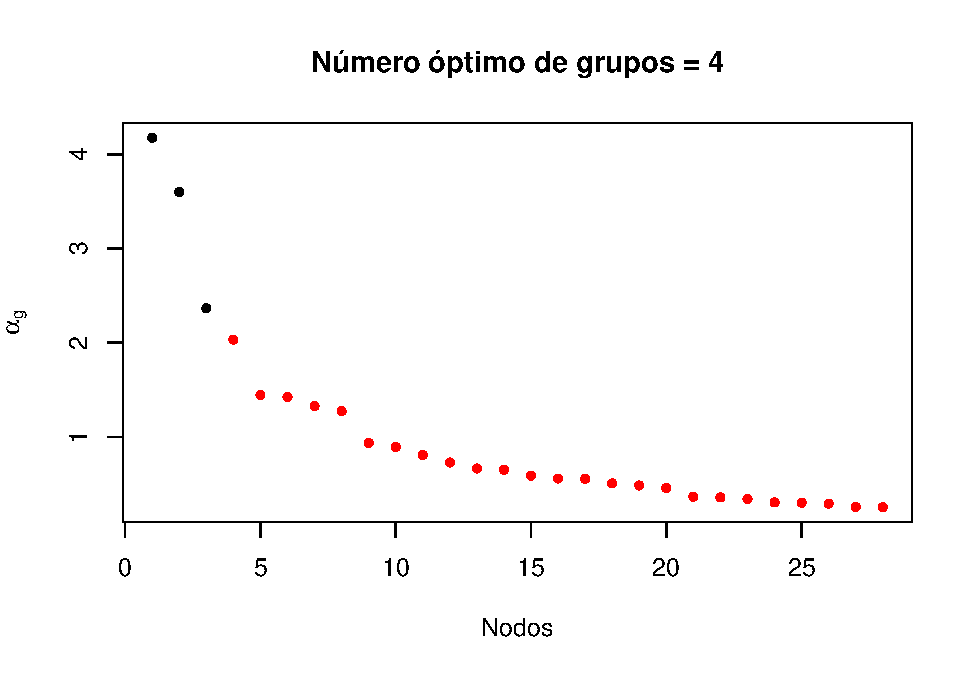
\includegraphics{4_actividad_cluster_files/figure-latex/Mojena-1.pdf}
\caption{Gráfica de Mojena para identificación de número óptimo de
conglomerados}
\end{figure}

Se comprueba esto a través del método del \emph{codo} el cual se muestra
en la figura 9. Este método define que el número de aglomerados es
aquellos que estén dentro de la suma de los cuadrados, en el punto de
inflexión dónde esta suma no aporte más información. Al aplicar este
método se puede observar nuevamente que el número de aglomerados más
adecuado para este conjunto de datos es 4.

\begin{figure}
\centering
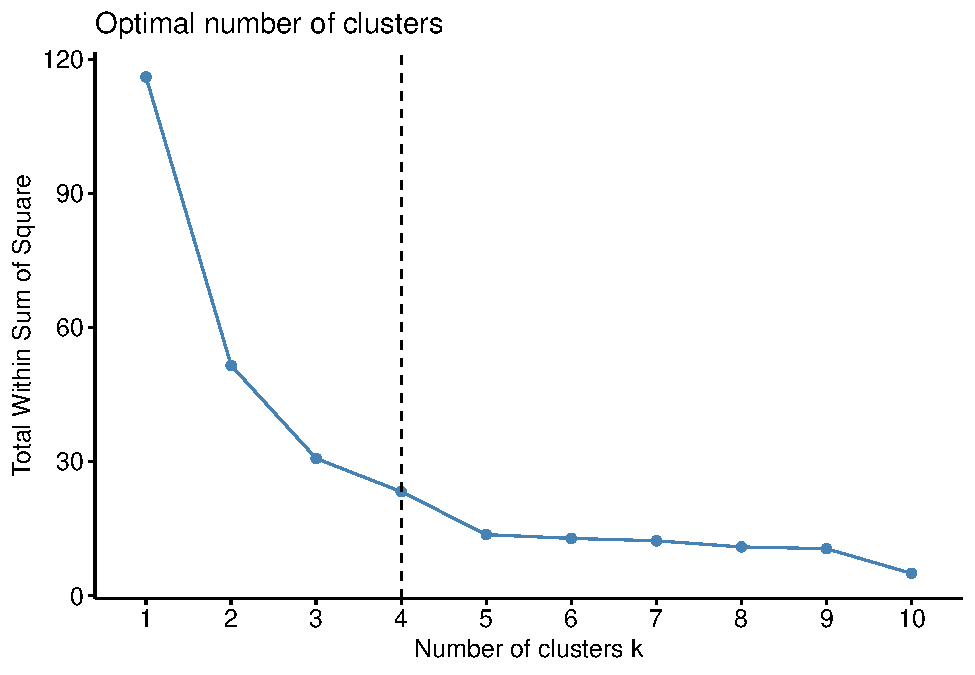
\includegraphics{4_actividad_cluster_files/figure-latex/definiendo conglomerados por wss-1.pdf}
\caption{Gráfica para definición de número de conglomerados para
\(K-medias\) por método WSS (within-cluster sum of square)}
\end{figure}

Definido el número de aglomerados, se procede a gráficar estos a través
del método de K-medias (figura 10). Esta figura llama la atención
encuanto define los 4 aglomerados, donde uno de estos está conformada
por una única observación, esta corresponde a \texttt{Greece} esto
quiere decir lo que se ha visto anteriomente que este país presenta una
problemática en cuanto a resistencia antibiótica muy particular que no
se relaciona con los comportamientos de los demás países. Además se
puede observar que el conglomerado 3 (gris), agrupa principalmente
países de europa del sur y oriente y su aporte lo realizan en la primera
componente principal, esto indica que estos países son los que más
aportan a la resistencia atibiótica en Europa (junto a Grecia) en
especial a antibióticos como las \texttt{Aminoglucosides} y
\texttt{Cephalo\_3er\_gen}.

De igual manera, es interesante el análisis de los agrupamientos 2 y 4.
Claramente se observa que los países que corresponde al grupo 4, son
países del norte de europa y son países cuya contribución es poca para
la problemática de resistencia antibiótica. Los países del grupo 2,
principalmente de países de occidentales también tiene un escaso impacto
en la resistencia antibiótica, incluso se puede observar en este grupo
algunos páises de sur y oriente de europa. Sin embargo, se evidencia que
son países que son geográficamente más cercanos a países occidentales,
esto puede sugerir que los patrónes de resistencia en Europa presentan
un patrón geográfico partícular y que las acciones frente a la
resistencia a los atibióticos pueden ser más efectivas en países de
occidentales y del norte de europa.

\begin{figure}
\centering
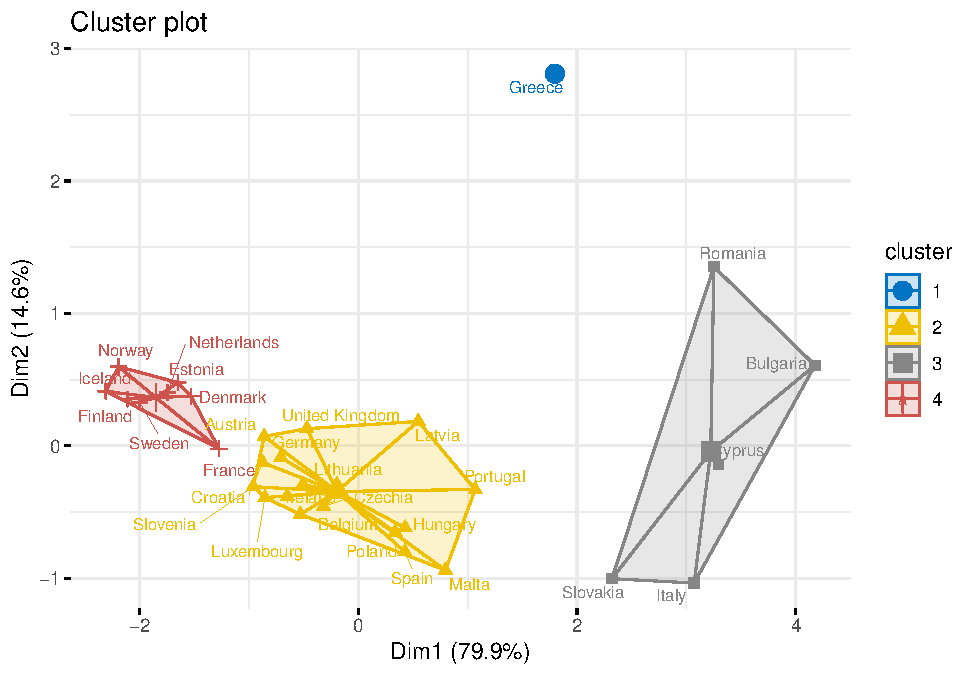
\includegraphics{4_actividad_cluster_files/figure-latex/conglomerados K medias para ecoli-1.pdf}
\caption{Gráfica de conglomerados por método de K-medias}
\end{figure}

\hypertarget{anexo-anuxe1lisis-de-conglomerados-k-medias-para-klebsiella-pneumoniae}{%
\subsection{\texorpdfstring{Anexo (análisis de conglomerados
(\(k\)-medias) para Klebsiella
Pneumoniae)}{Anexo (análisis de conglomerados (k-medias) para Klebsiella Pneumoniae)}}\label{anexo-anuxe1lisis-de-conglomerados-k-medias-para-klebsiella-pneumoniae}}

Para ampliar el análisis previo se decide realizar un estudio del
comportamiento entre países de la especie bacteriana \emph{Klebsiella
pneumoniae}, para evaluar si el comportamiento de resistencia los grupos
de antibióticos estudiados se asemeja al visto al ya descrito en el
análisis anterior de la \emph{Escherichia coli},

La figura 11. permite apreciar para la \emph{Klebsiella pneumoniae}
algunas similitudes con el mapa de calor de distancias descrito antes
para la otra bacteria. Sin embargo, en acá se ve que la distancias de
resistencia para Klebsiella en \texttt{Greece} dista de los demás países
en Europa. Esto concuerda con lo visto en el caso anterior.

\begin{figure}
\centering
\includegraphics{4_actividad_cluster_files/figure-latex/Distancis gráfica kelbsiella-1.pdf}
\caption{Matriz de distancias euclidianas para Klebsiella Pneumoniae}
\end{figure}

Se realiza un dendograma a través del método \emph{Average}
encontrandose nuevamente una fuerte distinción de aglomerados entre
países de sur y oriente de europa con relación a los de norte y
occidente, y nuevamente \texttt{Greece} se encuentra en una rama única
lo que sugiere su comportamiento único respecto a la resistencia
antibiótica de la Klebsiella.

\begin{figure}
\centering
\includegraphics{4_actividad_cluster_files/figure-latex/Método de Average para Klebisella-1.pdf}
\caption{Dendograma utilizando el método \emph{``Average''} para
Klebsiella Pneumoniae}
\end{figure}

Se decide aplicar el criterio de \emph{Mojena} (figura 13.)para definir
el número de aglomerados para definir en el método de \(K-medias\),
obteniendose 3 aglomerados, lo que es comprobado por el método del
\emph{codo}

\begin{figure}
\centering
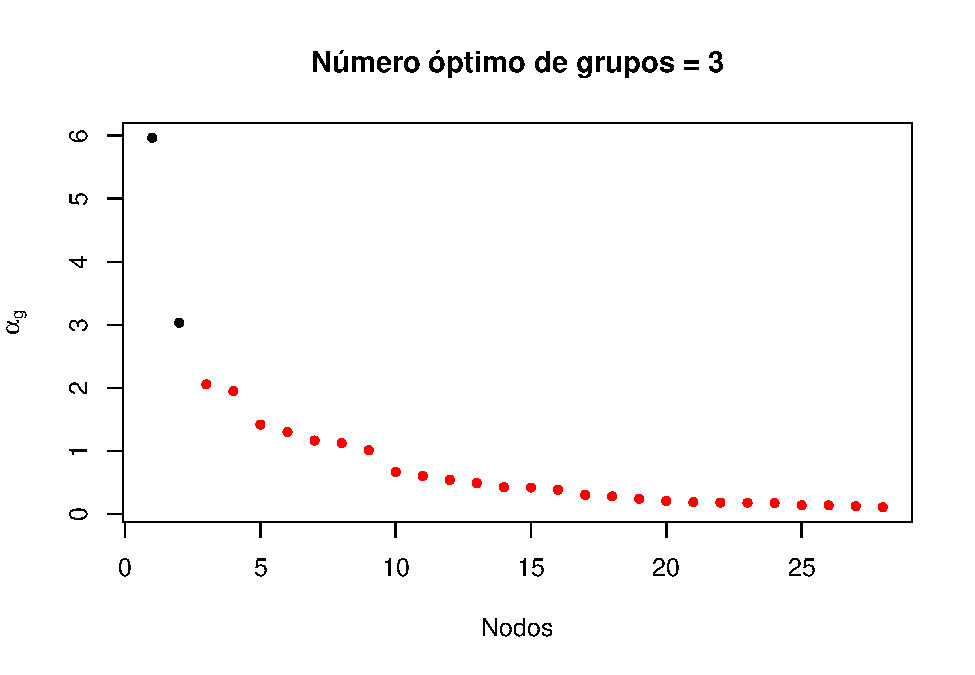
\includegraphics{4_actividad_cluster_files/figure-latex/Mojena Klebsiella-1.pdf}
\caption{Gráfica de Mojena para identificación de número óptimo de
conglomerados para Klebsiella Pneumoniae}
\end{figure}

A partir de la definición de estos tres aglomerados se decide gráficar
el método de \(K-medias\) con 25 iteraciones (figura 14.). Nuevamente se
observa un grupo propio para \texttt{Greece} es el mayor contribuidor
para la componente principal 1; esto indica que es el país que más
conribuye a la resistencia antibiótica de la \emph{Klebsiella
pneumoniae} para Fluoroquinolonas y cefalosporinas de 3er generación.
Además se evidenica que siguiente grupo que contribuye es el 2 (verde)
el cual está conformado por países de sur y oriente de europa y
nuevamente los países de norte y occidente son los que menos contribuyen
a esta problemática.

\begin{figure}
\centering
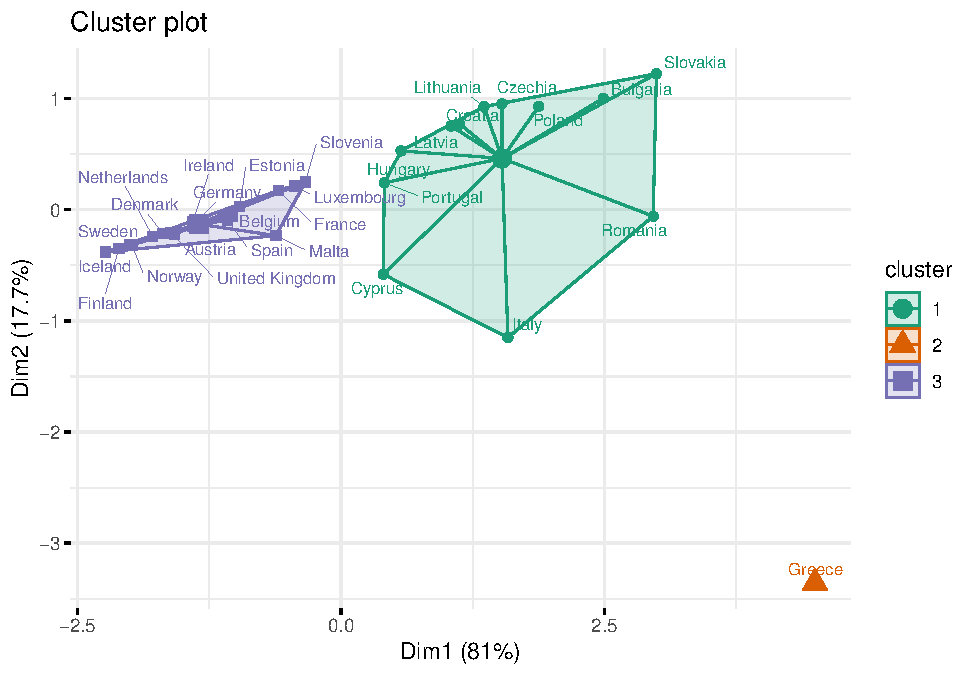
\includegraphics{4_actividad_cluster_files/figure-latex/conglomerados K medias para kpneumoniae-1.pdf}
\caption{Gráfica de conglomerados por método de K-medias para Klebsiella
Pneumoniae}
\end{figure}

\hypertarget{conclusion-y-perspectivas}{%
\subsection{Conclusion y perspectivas}\label{conclusion-y-perspectivas}}

\begin{itemize}
\item
  Los países del sur y oriente de europa son los que más contribuyen a
  la resistencia antibiótica tanto de \emph{Escherichia coli} como de la
  \emph{Klebsiella pneumoniae}. Se hizo una pequeña revisión de la
  literatura y se encontraron resultados similares para otros agentes
  infecciosos; por ejemplo, esta región es la que
  \href{https://www.cidrap.umn.edu/news-perspective/2017/11/latest-european-data-show-increasing-antibiotic-resistance}{más
  resistencia antibiótica en diferentes especies de
  \emph{Acinetobacter}}. Además recientemente se encontró que los países
  de estas regiones son las que más tienden a
  \href{https://aricjournal.biomedcentral.com/track/pdf/10.1186/s13756-019-0662-8}{utilizar
  antibióticos de última línea}. de manejo para agentes infecciososo
  como \emph{Pseudomonas aeruginosa} y diferentes especiedes de
  bacterias del genero \emph{Enterobacteriaceae}. Incluso
  \href{https://www.euro.who.int/en/health-topics/disease-prevention/antimicrobial-resistance/news/news/2019/7/survey-in-eastern-european-and-central-asian-countries-finds-further-control-of-antibiotics-use-needed}{la
  OMS (organización mundial de la Salud)}.ha previsto la gran necesidad
  de aunar esfuerzos para resolver la situación de resistenica
  antibiótica en estos páises
\item
  Dentro de los países sur-orientales de europa el que tiene un
  comportamiento más particular es Grecia. Parece que es el máximo
  contribuidor de resistencia antibiótica en las dos bacterias
  estudiadas, esto indica que sus comportamientos para el manejo
  antibiótico son distintas a las vistas en otros países. Esto se ha
  intentado explicar por un
  \href{https://www.bmj.com/content/355/bmj.i6328/rr-0}{abuso del uso de
  antibióticos} en diferentes escenarios clínicos en este país . No es
  la primera vez que se evidencia esto, ya múltiples grupos han
  encontrado
  \href{http://resistancecontrol.info/2016/government-engagement/national-strategies-for-the-control-of-antimicrobial-resistance-the-hellenic-challenge/}{resultados
  similares}. Sin embargo, las razones precisas de este efecto no son
  del todo claras y se requieren de más estudios de indole social,
  cultura y clínico par establecer este efecto.
\item
  En el análisis llevado acabo en esta actividad se evidencia que en la
  medida que los países sur-orientales de europa se acercan
  geográficamente al occidente o el norte de europa sus frecuencias de
  resistencia antibiótica es menor. Esto debe ser comprobado a través de
  más estudios geopoblacionales. Sin embargo, permite lanzar supuestos
  respecto a la conciencia acerca del uso racional de los antibióticos
  en occidente y también a las mayores prácticas de regulación y control
  que se han adoptado en muchos países de europa occidental para
  contener esta problemática de caracter mundial.
\end{itemize}

\end{document}
